% ~~~ [ Control Flow Analysis ] ~~~~~~~~~~~~~~~~~~~~~~~~~~~~~~~~~~~~~~~~~~~~~~~~

\subsubsection{Control Flow Analysis}
\label{sec:lit_review_control_flow_analysis}

Control Flow Graph (CFG)

foo

% TODO: Add notes about irriducible graphs; may be solved using node splitting.
% * functional (semantics?) vs. forensic equivalence.

\begin{figure}[htbp]
	\centering
	% if
	\begin{subfigure}[ht]{0.23\textwidth}
		\centering
		\begin{subfigure}[ht]{0.45\textwidth}
			\lstinputlisting[language=go, style=go, breaklines=false, numbers=none]{inc/primitives/if.c}
		\end{subfigure}
		\begin{subfigure}[ht]{0.42\textwidth}
			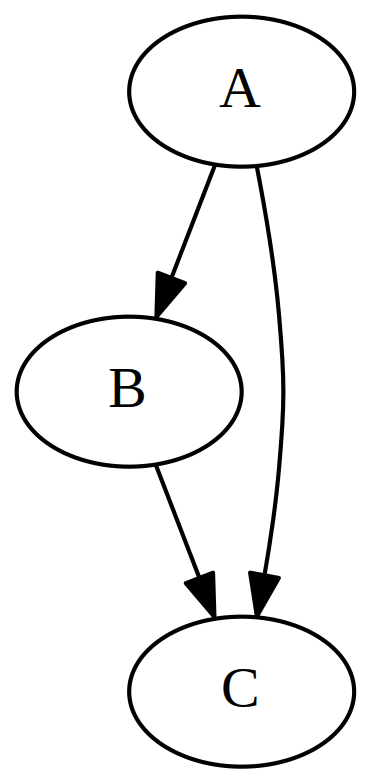
\includegraphics[width=\textwidth]{inc/primitives/if.png}
		\end{subfigure}
		\caption{1-way conditional; entry: \texttt{A}, exit: \texttt{C}.}
		\label{fig:if_graph_representation}
	\end{subfigure}
	\qquad
	% if_else
	\begin{subfigure}[ht]{0.28\textwidth}
		\centering
		\begin{subfigure}[ht]{0.45\textwidth}
			\lstinputlisting[language=go, style=go, breaklines=false, numbers=none]{inc/primitives/if_else.c}
		\end{subfigure}
		\begin{subfigure}[ht]{0.50\textwidth}
			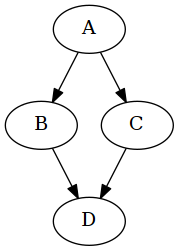
\includegraphics[width=\textwidth]{inc/primitives/if_else.png}
		\end{subfigure}
		\caption{2-way conditional; entry: \texttt{A}, exit: \texttt{D}.}
		\label{fig:if_else_graph_representation}
	\end{subfigure}
	\qquad
	% if_return
	\begin{subfigure}[ht]{0.30\textwidth}
		\centering
		\begin{subfigure}[ht]{0.45\textwidth}
			\lstinputlisting[language=go, style=go, breaklines=false, numbers=none]{inc/primitives/if_return.c}
		\end{subfigure}
		\begin{subfigure}[ht]{0.50\textwidth}
			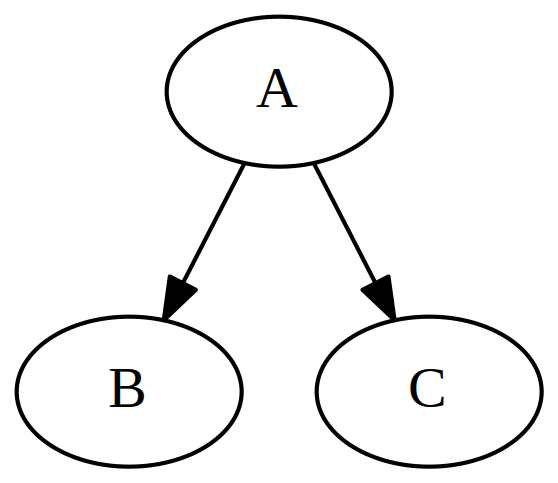
\includegraphics[width=\textwidth]{inc/primitives/if_return.png}
		\end{subfigure}
		\caption{1-way condition with return statement in body; entry: \texttt{A}, exit: \texttt{C}.}
		\label{fig:if_return_graph_representation}
	\end{subfigure}
	\qquad
	% pre_loop
	\begin{subfigure}[ht]{0.32\textwidth}
		\centering
		\begin{subfigure}[ht]{0.45\textwidth}
			\lstinputlisting[language=C, style=go, breaklines=false, numbers=none]{inc/primitives/pre_loop.c}
		\end{subfigure}
		\begin{subfigure}[ht]{0.50\textwidth}
			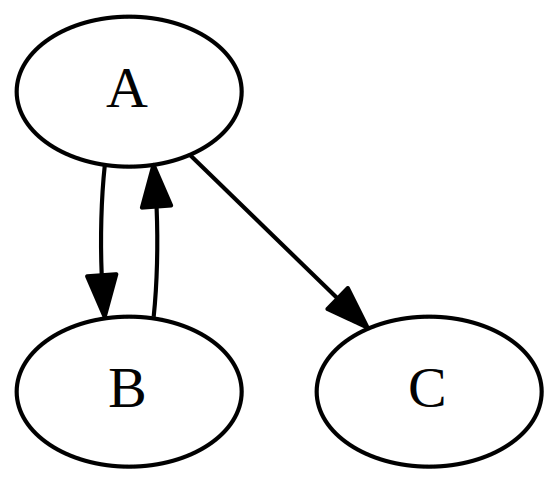
\includegraphics[width=\textwidth]{inc/primitives/pre_loop.png}
		\end{subfigure}
		\caption{pre-test loop; entry: \texttt{A}, exit: \texttt{C}.}
		\label{fig:pre_loop_graph_representation}
	\end{subfigure}
	\qquad
	% post_loop
	\begin{subfigure}[ht]{0.30\textwidth}
		\centering
		\begin{subfigure}[ht]{0.50\textwidth}
			\lstinputlisting[language=C, style=go, breaklines=false, numbers=none]{inc/primitives/post_loop.c}
		\end{subfigure}
		\begin{subfigure}[ht]{0.35\textwidth}
			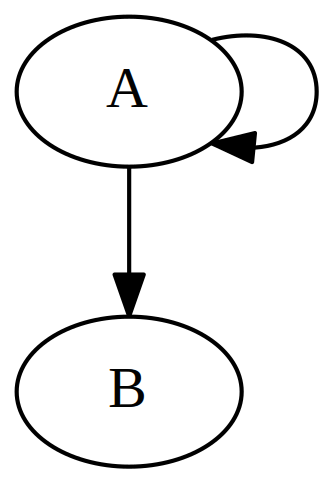
\includegraphics[width=\textwidth]{inc/primitives/post_loop.png}
		\end{subfigure}
		\caption{post-test loop; entry: \texttt{A}, exit: \texttt{B}.}
		\label{fig:post_loop_graph_representation}
	\end{subfigure}
	\qquad
	% list
	\begin{subfigure}[ht]{0.24\textwidth}
		\centering
		\begin{subfigure}[ht]{0.20\textwidth}
			\lstinputlisting[language=C, style=go, breaklines=false, numbers=none]{inc/primitives/list.c}
		\end{subfigure}
		\begin{subfigure}[ht]{0.35\textwidth}
			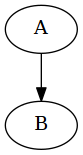
\includegraphics[width=\textwidth]{inc/primitives/list.png}
		\end{subfigure}
		\caption{consecutive statements; entry: \texttt{A}, exit: \texttt{B}.}
		\label{fig:list_graph_representation}
	\end{subfigure}
	\caption{The pseudo-code and graph representation of various high-level control flow primitives with denoted entry and exit nodes.}
	\label{fig:graph_representations}
\end{figure}
